\section*{Question 2:}
Exercise 10.5: 

Find a community-based question answering site on the Web and ask two questions, one that is low-quality and one that is high-quality. Describe the answer quality of each question.

\subsection*{Answer:}

I chose to use Yahoo! Answers and asked the following question as a high quality one:


Will Turkey leave NATO and form a coalition with Russia and Iran after US backed Syrian Kurds and moved US embassy in Tel Aviv to Jerusalem?

I consider this as a high quality question because of its correct grammar and punctuation. It also targets the kind of users that care about politics who are normally serious people. The question is about the possibility of a certain outcome as a result of current events. The answer should be definitive, either yes or no.

Below is a screen shot of the answers I got:


\begin{figure}[h]
\caption{Answers for high quality question}
\centering
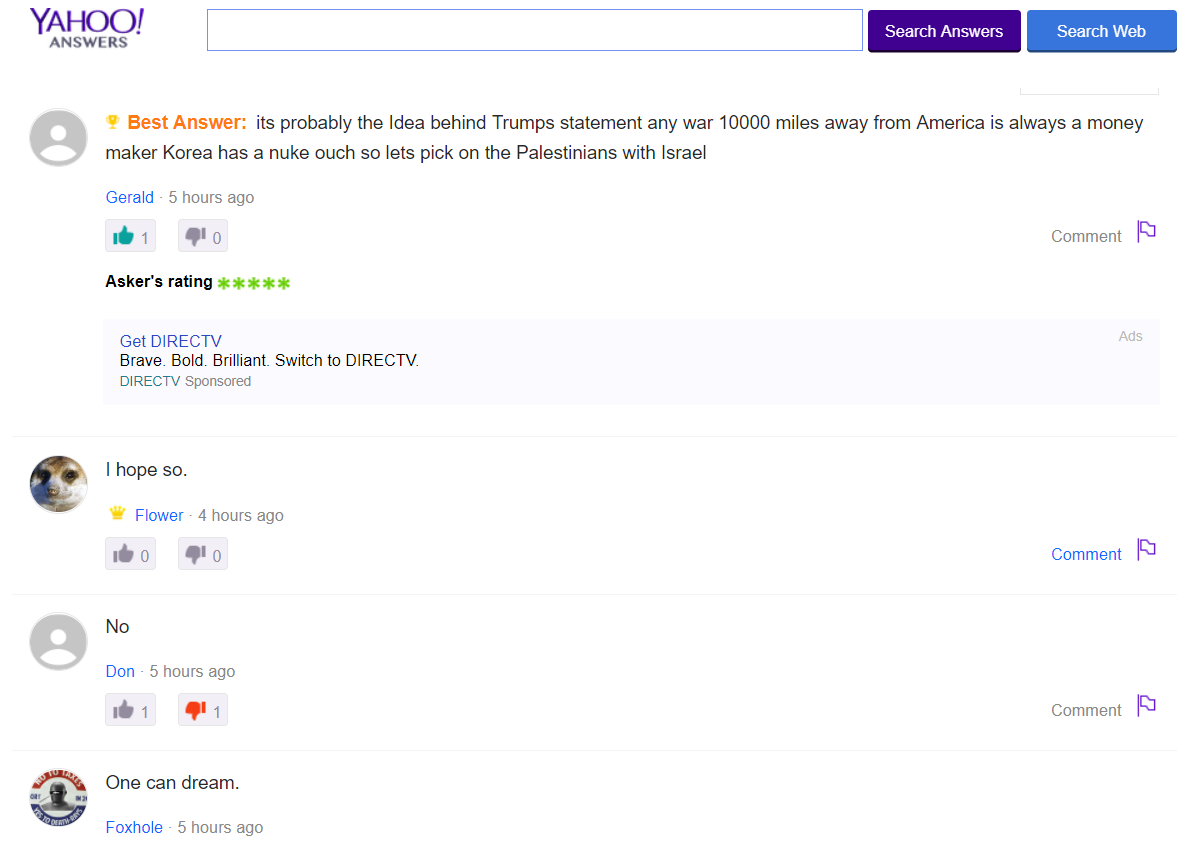
\includegraphics[scale=0.6]{Q2/high.png}
\end{figure}


I marked the answer that has a short analysis of why Turkey might leave NATO as best answer. The answers are high quality and meant to answer the question, but they are short, which is expected.  

I asked the following question as a low quality one: 

Why did you Trump to helb tha kill Saudi to Yemen? Are you forget wat hapend at 11 septemper? Saudi mans kil 3000 America at airplain atak.?

I discovered that asking a low quality question is not an easy task. I was finally able to do it by writing a question then injecting/removing pronouns, verbs, and preposition to produce wrong grammar. I also misspelled some words to make it worse. 

Below is a screen shot of the answers I got:


\begin{figure}[h]
\caption{Answers for low quality question}
\centering
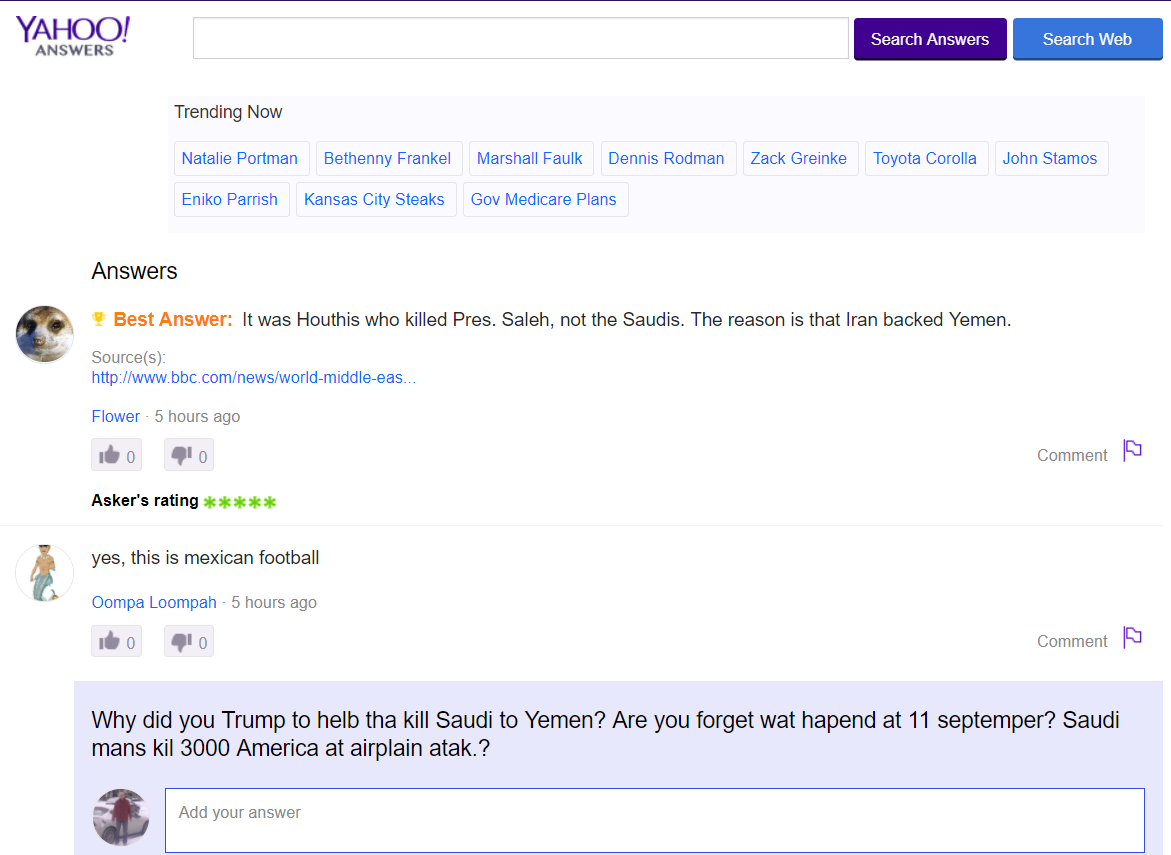
\includegraphics[scale=0.6]{Q2/low.png}
\end{figure}


Surprisingly, I got an answer that is, to a certain extent, related to the topic of the question. I would call that a high quality answer because I do not think that it is possible to come up with a much better answer. The answer includes a source link from BBC. 

For the other answer, I thought that was funny, but it turns out that Yahoo! put my question in the Mexican football category within sports, and that explains why I got this answer. It is, of course, a low quality answer, and it is definitely not related to the question.

\textbf{Observation:}

The results were as expected; low quality questions get low quality answers, and high quality questions get high quality answers.
